\documentclass[12pt,a4paper]{article}
\usepackage{ucs}
\usepackage[utf8x]{inputenc}
\usepackage{amsmath}
\usepackage{graphicx}
\usepackage{wrapfig}

\title{Osnove Mehatronike 2. lab}
\newcommand{\brvjezbe}{2}
\newcommand{\ime}{Niko Višnjić}
\newcommand{\jmbag}{0036449299}
\newcommand{\grupa}{unknown}
\newcommand{\predmet}{Osnove mehatronike} 
\newcommand{\fakultet}{Fakultet elektrotehnike i računarstva Zagreb} 
\newcommand{\zavod}{Zavod za elektrostrojarstvo i automatizaciju } 
\newcommand{\imevjezbe}{Vježba 2: Regulacija brzine vrtnje rotacijskog elektromehaničkog sustava SRV02\newline
- sinteza regulatora -}
\usepackage[hmargin={3.5cm,2.5cm},height=25.5cm]{geometry}
\input{"zaglavlje.tex"}
\setcounter{secnumdepth}{4}

\DeclareMathSizes{12}{12}{10}{12}

\begin{document}
\section{Uvod}
U okviru ove vježbe obavljamo sintezu regulatora brzine vrtnje rotacijskog elektromehaničkog sustava SRV02 i njegovu simulaciju na par specifičnih primjera.

Vježba se sastoji od dva pokusa.
U prvom stvaramo matematički model rotacijskog elektromehaničkog modula sustava SRV02, te određujemo parametre regulatora procesa. U drugom dijelu uzimamo napravljeni model procesa te simuliramo njegove odzive na skokovitu pobudu uz različite parametre regulatora i samog procesa.Vježbu izvodimo u MATLAB/Simulink programskom okruženju.
U nastavku dokumentiramo i opisujemo pokuse te bilježimo dobivene rezultate i naša zapažanja iz dobivenih mjerenja.

\newpage

\section{Pokusi}
\subsection{Pokus 1 : Određivanje parametara regulatora brzine vrtnje rotacijskog elektromehaničkog sustava SRV02}

Zadatak je da se korištenjem Matlab-a projektira regulator brzine vrtnje rotacijskog elektromehaničkog sustava SRV02, koji će zadovoljiti kriterije navedene u poglavlju~\ref{sec:zahtjevi}.

Kako bi uopće mogli pristupiti sintezi regulatora, moramo imati matematički model našeg elektromehaničkog rotacijskog modula SRV02. Njegovo definiranje opisano je u nastavku.

\subsubsection{Matematički model rotacijskog elektromehaničkog sustava SRV02}
Uzevši u obzir zakone kinematike te korištenjem Kirchoffovih zakona za električki model motora prikazan na slici 2.1, i primjenom određenih zanemarenja, dobivamo sljedeći sustav jednadžbi.

\begin{figure}[h]
	\begin{center}
	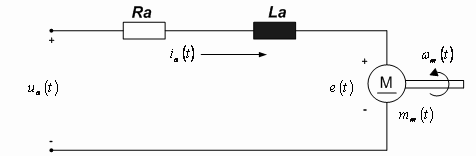
\includegraphics[width=0.8\textwidth] {ele_motor.png}
    \caption{Nadomjesna shema naponom upravljanog istosmjernog motora}
    \end{center}
\end{figure}

\begin{equation}
 i_a=\frac{u_a-k_e\omega_m}{R_a}
\end{equation}

\begin{equation}
 J_m\frac{\mathrm{d}\omega_m}{\mathrm{d}t}=m_m - \frac{m_t}{\eta_gK_g}
\end{equation}

\begin{equation}
J_t\frac{\mathrm{d}\omega_t}{\mathrm{d}t}=m_t - B_{eq}\omega_t
\end{equation}

Iz sustava jedadžbi slijedi prijenosna funckija prvog reda koja opisuje elektromehanički sustav:

\begin{equation}
G(s)=\frac{\omega_t(s)}{u_a(s)}=\frac{\eta_g\eta_mk_mK_g}{J_{eq}R_as + B_{eq}R_a+\eta_g\eta_mk_ek_mK_g^2}
\end{equation}

gdje \begin{equation}J_{eq}=J_t+\eta_gJ_mK_g^2\end{equation}
Izraz (2-5) opisuje ukupni (ekvivalentni) moment inercije reduciran na stranu tereta.

\newpage


\subsubsection{Prikaz matematičkog modela SRV02 u Simulink okruženjuj}
Navedenu prijenosnu funkciju možemo izraziti nadomjesnom shemom u Simulink okruženju prema modelu prikazanom na slici 2.2.

\begin{figure}[h]
	\begin{center}
	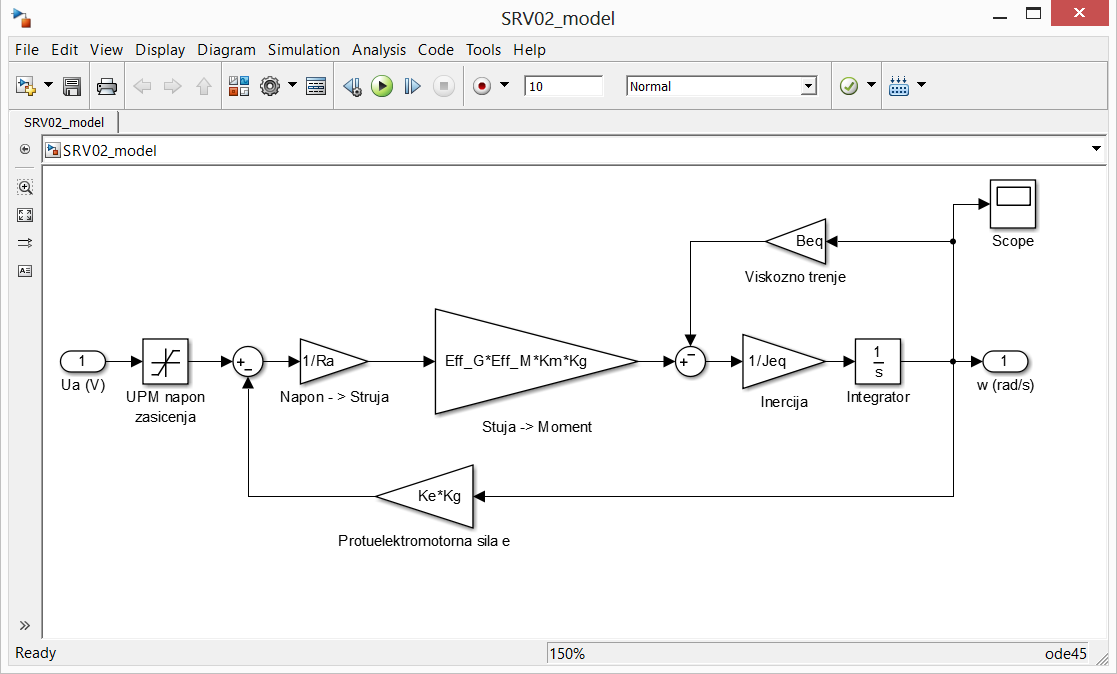
\includegraphics[width=0.8\textwidth] {model.png}
    \caption{Simulink model elektromehaničkog sustava SRV02}
    \end{center}
\end{figure}


\subsubsection{Regulacijski zahtjevi}
\label{sec:zahtjevi}
Zadatak je projektirati sustav regulacije brzine s PD kompenzatorom sa ciljem upravljanja rotacijskim elektromehaničkim sustavom SVR02 sa sljedećim zahtjevima:

\begin{itemize}
  \item Sustav treba imati statičku pogrešku jednaku nuli
  \item Presječna frekvencija sustava treba iznositi 100 rad/s (otprilike 16 Hz)
  \item Otvoreni sustav treba imati fazno osiguranje približno 75 stupnjeva
  \item Sustav ne smije imati nadvišenje
\end{itemize}

\newpage

\subsubsection{Sinteza regulatora}
Kod sinteze sustava regulacije brzine s PD kompenzatorom u frekvencijskoj domeni potrebno je proučiti Bodeove frekvencijske karakteristike otvorenog kruga. U nastavku opisujemo postupak sinteze komponenata regulatora da bi ispunili regulacijske zahtjeve koji su nam dati iznad.

\paragraph{Statička pogreška}
Kako bi ispunili prvi regulacijski zahtjev, odnosno da bi imali statičku pogrešku sustava jednaku nuli (na skokovitu ulaznu funkciju), moramo imati astatizam prvog reda. Astatički sustav sadrži jedan ili više integralnih članova,a a njihov broj određuje red astatizma.

Uvrštavanjem vrijednosti parametara, navedenih u Dodatku 1. za drugu laboratorijsku vježbu, u jednadžbu (2-4) dobivamo konačnu vrijednost prijenosne funkcije sustava, odnosno prijenosnu funkciju procesa sustava.

\begin{equation}
G_p(s)=\frac{0.066796}{2.5441\cdot10^{-4}\cdot s + 0.01107966}
\end{equation}


Po definicji, sustav je astatički prvog reda ukoliko ima jedan pol smješten u ishodištu. Kako vidimo, prijenosna funkcija ne odgovara toj definiciji. Da bi postigli astatizam prvoga reda, potrebno je uvesti integracijski član u regulacijski krug.


Uvrštavanjem regulatora dobivamo prijenosnu funkciju otvorenog regulacijskog kruga s integratorom $G_p(s)/s$, čiji je Bodeov dijagram prikazan na slici 2.3.

\begin{figure}[h]
	\begin{center}
	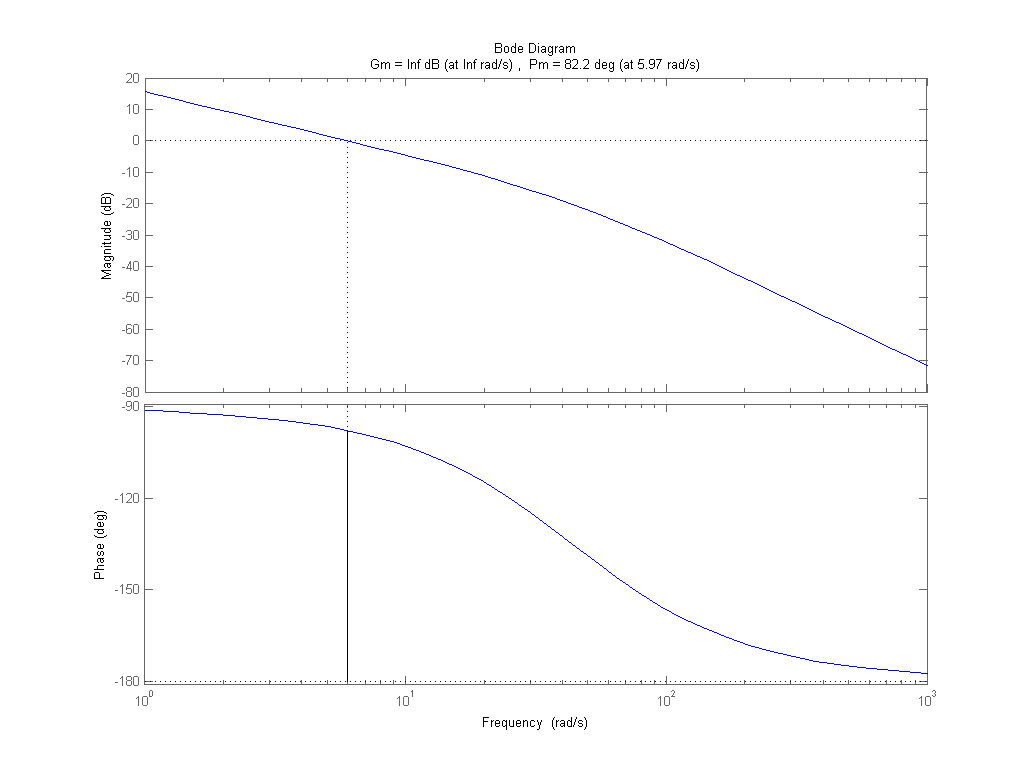
\includegraphics[width=0.8\textwidth] {bode_1.png}
    \caption{Bodeov dijagram otvorenog kruga s integratorom $G_p(s)/s$}
    \end{center}
\end{figure}

\newpage

\paragraph{Podešavanje pojačanja $K_p$}
Kako bi ispunili sljedeći zahtjev regulacije, pri kojemu moramo namjestiti da presječna frekvencija sustava iznosi približno 100 rad/s, množimo prijenosnu funkciju otvorenog regulacijkog kruga s dodanim integracijskim članom s konstantom pojačanja $K_p$. Točnu vrijednost konstante Kp određujemo iterativnim postupkom, dok ne dobijemo da pojačanje sustava iznosi 0 dB, odnosno 1, pri frekvenciji od 100 rad/s.

Dobivamo da je tražen iznos statičkog pojačanja $K_p = 41.55$. Na slici 2.4 možemo vidjeti Bodeov dijagram prijenosne funkcije otvorenog regulacijskog kruga s dodanim integratorom i pojačanjem $K_p\cdot G_p(s)/s$.

\begin{figure}[h]
	\begin{center}
	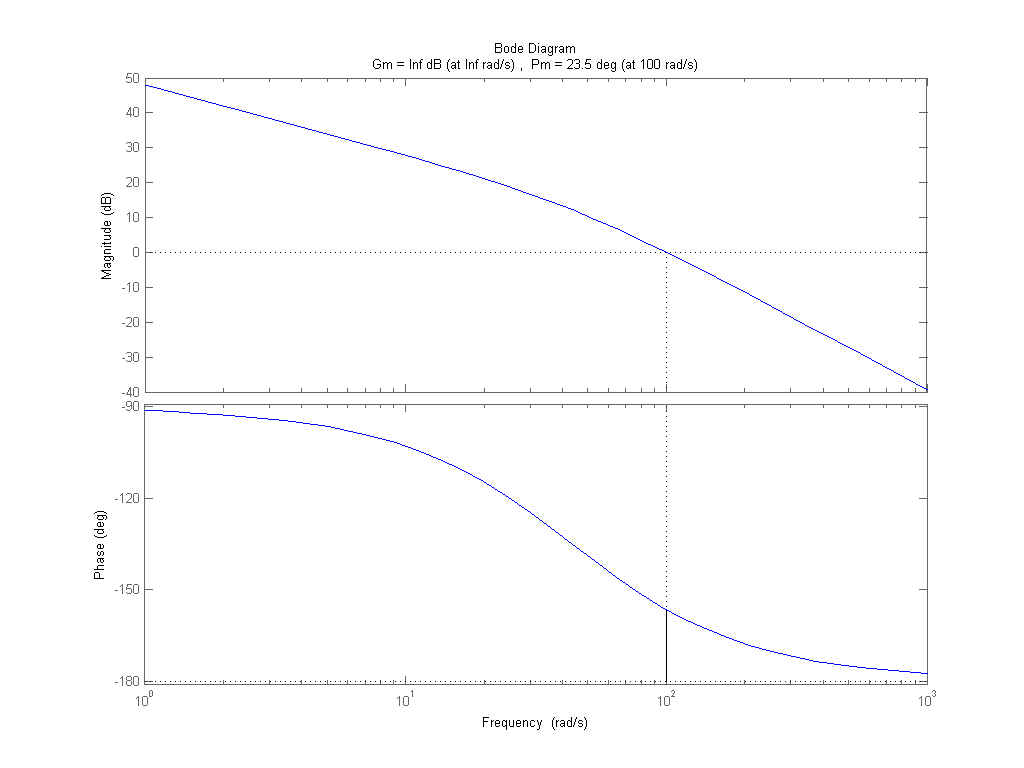
\includegraphics[width=0.8\textwidth] {bode_2.png}
    \caption{Bodeov dijagram otvorenog kruga s integratorom i pojačanjem $K_p\cdot G_p(s)/s$}
    \end{center}
\end{figure}

\paragraph{Projektiranje derivacijskog kompenzacijskog člana}
Derivacijski kompenzacijski član služi za korekciju Bodeove fazne karakteristike promatranog sustava. Potrebno je projektirati derivacijski kompenzacijski član koji će unijeti traženi fazni pomak u gasnoj karakteristici pri čemu presječna frekvencija mora ostati nepromjenjena, odnosno pojačanje kompenzacijskog člana na presječnoj frekvenciji mora biti 0 dB, odnosno 1. Derivacijski kompenzacijski član općenito ima prijenosnu funkciju oblika:

\begin{equation}
C(s)=\alpha\frac{s+\frac{\omega_c}{\alpha}}{s+\alpha\omega_c}
\end{equation}

gdje je $\omega_c$ presječna frekvencija, a $\alpha$ parametar koji se računa kao:

\begin{subequations}
\begin{align}
	\tau_p &= tan\Phi\\
	\alpha &= \tau_p + \sqrt{\tau_p^2+1}
\end{align}
\end{subequations}

Kut $\Phi$ predstavlja kut za koji je potrebno korigirati faznu karakteristiku sustava.

Kako bi ispunili uvjet da fazno osiguranje našeg sustava iznosi $75^\circ$ i time ujedno i uvjet da smo sigurni da naš sustav neće imati nadvišenja, računamo za koliko je potrebno korigirati faznu karakteristiku sustava. Pogledom na sliku 2.4 vidimo da je trenutno fazno osiguranje sustava $\varphi = 23.5^\circ$, te uvrštavanjem ovih vrijednosti u (2-8a) i (2-8b) dobivamo:

\begin{align*}
\alpha &=  tan(75^\circ-\varphi) + \sqrt{tan^2(75^\circ-\varphi)+1}\\
	   &=2.8636
\end{align*}

i znajući da je tražena presječna frekvencija jednaka $\omega_c=100$ rad/s, iz (2-7) slijedi

\begin{equation}
C(s)=\frac{2.864\cdot s+100}{s+286.4}
\end{equation}


\paragraph{Regulirani sustav}
Time smo dobili i zadnju komponentu našeg regulacijskog kruga, te kombinacijom integracijskog člana, statičkog pojačanja $Kp$ i derivacijskog kompenzacijskog člana $C(s)$, dobivamo sustav koji ispunjava kriterije opisane u ~\ref{sec:zahtjevi}. 

Bodeov dijagram sustava s potpunim regulatorom $C(s)\cdot K_p\cdot G_p(s)/s$ možemo vidjeti na slici 2.5.

\begin{figure}[h]
	\begin{center}
	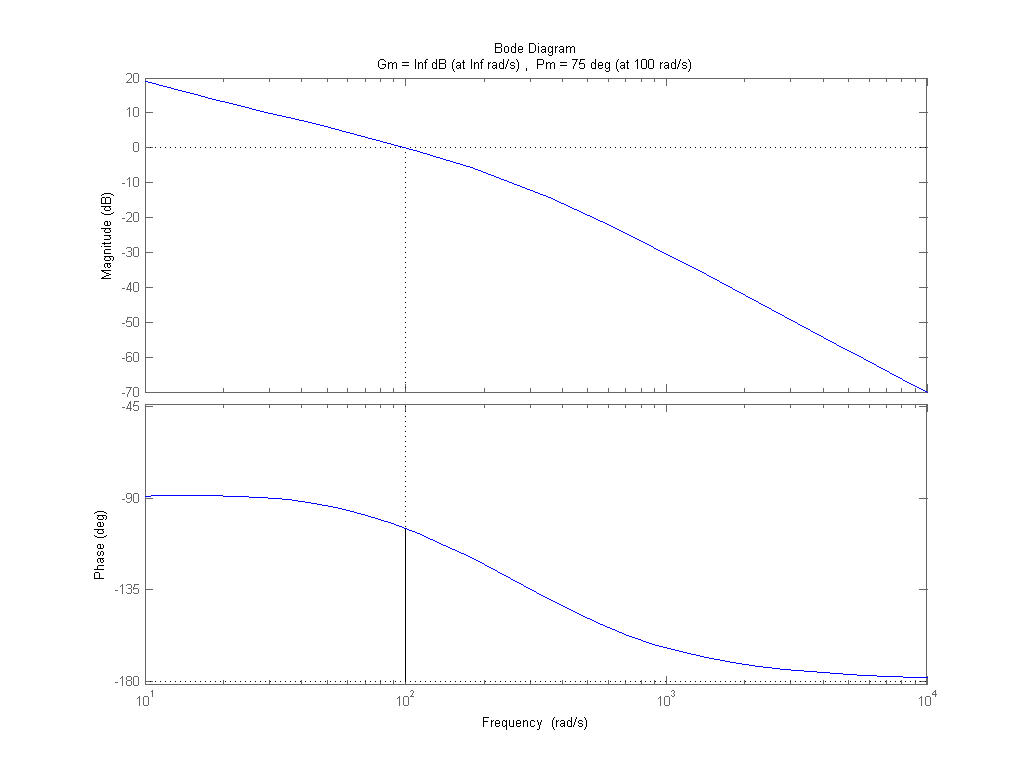
\includegraphics[width=0.8\textwidth] {bode_3.png}
    \caption{Bodeov dijagram otvorenog kruga s integratorom, pojačanjem te derivacijskim kompenzacijskim članom $C(s)\cdot K_p\cdot G_p(s)/s$}
    \end{center}
\end{figure}


\newpage

\subsubsection{Opažanja i zaključci}
Matematički model rotacijskog modula SRV02, odnosno proces, u ovom pokusu je statički. Da bi udovoljili kriterijima regulacije u pogledu da sustav u cijelini nema trajno regulacijsko odstupanje pri skokovitoj pobudi, morali smo sustavu dodati integrator u regulacijski krug. Time smo postigli astatizam prvog reda i anulirali statičku pogrešku našeg sustava.

Ukoliko bi promjenili pobudu iz step funkcije u konstantnu rampu, time bi se i astatizam sustava promjenio, odnosno dobili bi sustav s konstantnom (brzinkom) pogreškom. Primjer odziva sustava na takvu pobudu možemo vidjeti na slici 2.6.

\begin{figure}[h]
	\begin{center}
	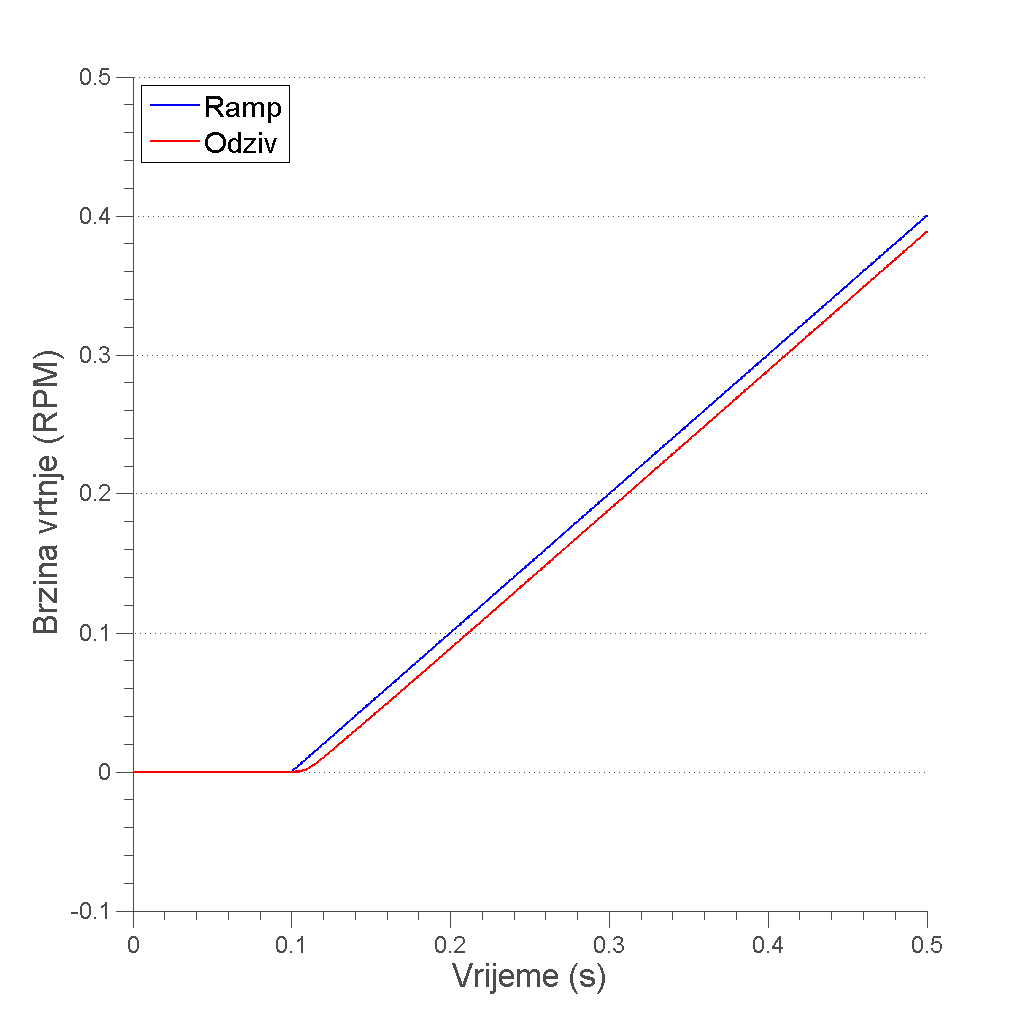
\includegraphics[width=0.8\textwidth] {ramp.png}
    \caption{Odziv sustava $C(s)\cdot K_p\cdot G_p(s)/s$ na funkciju linearnog porasta (ramp)}
    \end{center}
\end{figure}

Ukoliko želimo izračunati iznos regulacijskog odstupanja, odnosno brzinske pogreške $e_\infty$ koristimo se sljedećim formulama:

\begin{equation}
e_\infty=\lim_{s \to \infty} s \frac{1}{1 + G_o(s)}R(s)=\lim_{s \to \infty} \frac{1}{1 + G_o(s)}\frac{R}{s^2}=\frac{R}{K_0}
\end{equation}

\begin{equation}
K_0=\lim_{s \to \infty}sG_o(s)=K_p\frac{\eta_g\eta_mk_mK_g}{\alpha(B_{eq}R_a+\eta_g\eta_mk_ek_mK_g^2)}=88.5
\end{equation}

Te, za dati primjer, gdje je nagib funckije linearnog porasta jednak $R=1$, dobivamo da regulacijsko odstupanje iznosi $e_\infty=0.01129$

U ovom pokusu iste rezultate mogli smo postići koristeći PID regulator, gdje bi mu parametre odredili pomoću integralnih kriterija ili koristeći Zeigler-Nicholsove uvjete.


\newpage

\subsection{Pokus 2: Simulacija kruga regulacije brzine vrtnje rotacijskog elektromehaničkog sustava SRV02 }

Nakon određivanja parametara regulatora potrebno je simulirati krug  regulacije brzine vrtnje kako bi se potvrdilo da taj krug ispunjava kriterije postavljene u poglavlju ~\ref{sec:zahtjevi}.
Zadatak je:

\begin{itemize}
  \item Unutar Simulink okruženja načiniti odgovarajući simulacijski model sustava regulacije brzine vrtnje rotacijskog elektromehaničkog modula SRV02.
  \item Snimiti karakteristične odzive na skokovitu pobudu te potvrditi valjanost projektiranih parametara regulatora.
\end{itemize}


\subsubsection{Simulacijski model}
Unutar Simulink programskog okruženja definiramo model pomoću kojega ćemo simulirati krug regulacije brzine vrtnje rotacijskog elektromehaničkog sustava SRV02, kojeg smo odredili u prijašnjem pokusu.
Simulacijski model možemo vidjeti na slici 2.7.

\begin{figure}[h]
	\begin{center}
	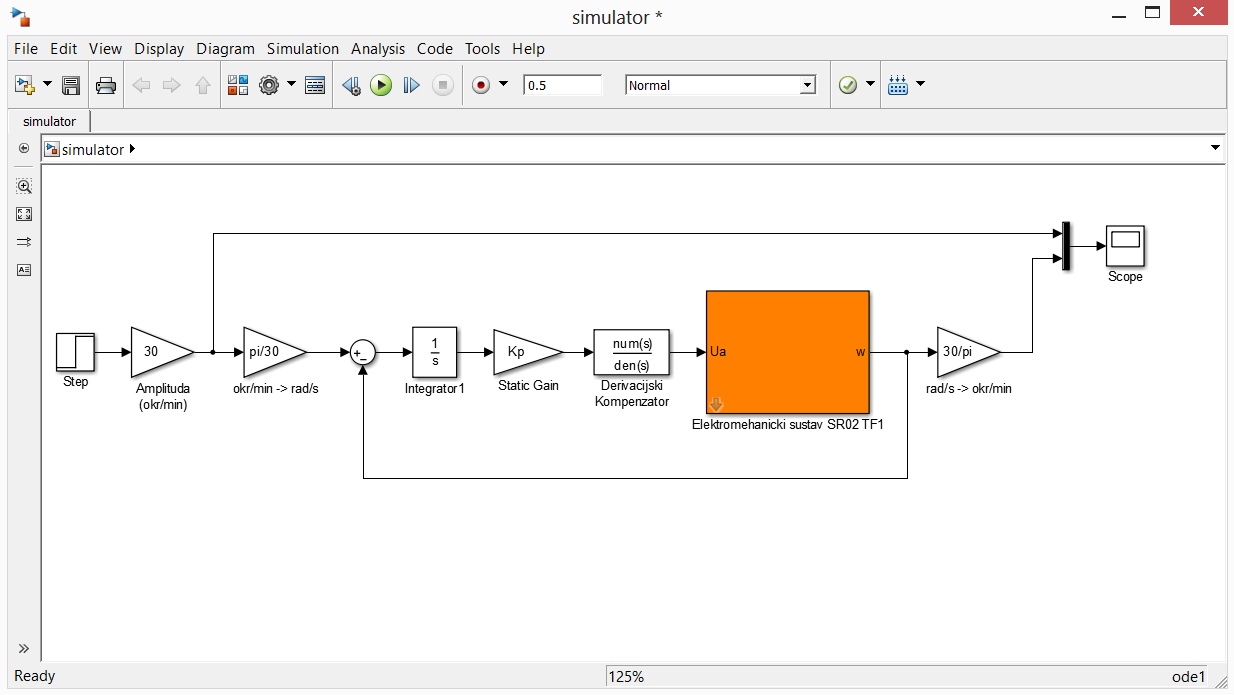
\includegraphics[width=0.8\textwidth] {simulator.png}
    \caption{Simulacijski model sustava regulacije brzine vrtnje rotacijskog elektromehaničkog modula SRV02}
    \end{center}
\end{figure}

Postavljanjem parametara modela prema Dodatku 1. iz uputa za drugu laboratorijsku vježbu, prelazimo na dobivene rezultate.

\newpage

\subsubsection{Rezultati simulacije}
U simulaciji uspoređujemo signale brzine vrtnje, gdje kao ulaznu pobudu imamo step funkciju, a kao izlaznu imamo odziv našeg reguliranog procesa na referentnu step funkciju.

Odziv sustava, kao što je definiran u prvom pokusu, vidimo na slici 2.8.

\begin{figure}[h]
	\begin{center}
	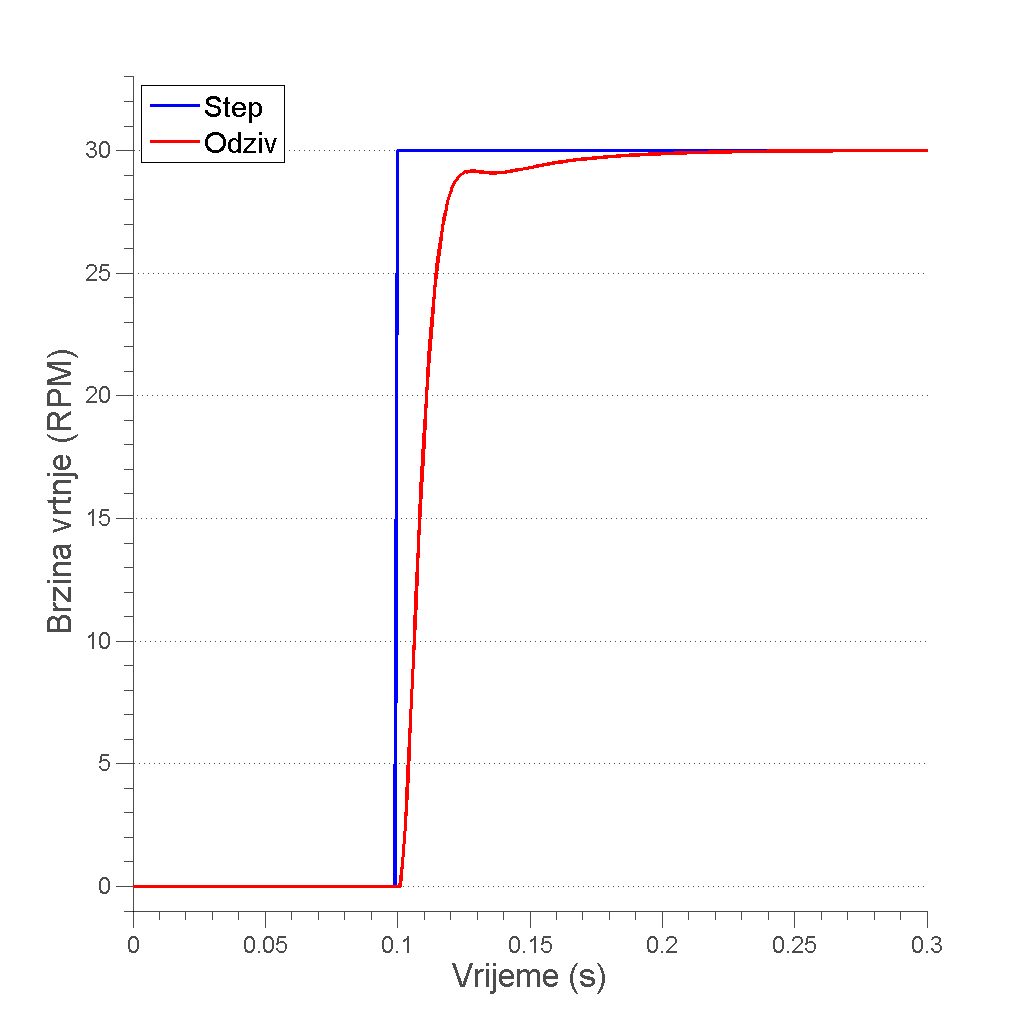
\includegraphics[width=0.8\textwidth] {odziv_1.png}
    \caption{Odziv sustava $C(s)\cdot Kp\cdot G_p(s)/s$ na skokovitu pobudu}
    \end{center}
\end{figure}

Primjećujemo da sustav dobro prati referentni signal nakon što se odziv ustali, odnosno da nema regulacijskog odstupanja te da sustav nema nadvišenja, kao što je i bilo zadano u regulacijskim zahtjevima sustava u poglavlju ~\ref{sec:zahtjevi}.


\newpage

Ukoliko sustavu oduzmemo integracijski član iz regulatora, dobivamo odziv kao što je prikazan na slici 2.9.


\begin{figure}[h]
	\begin{center}
	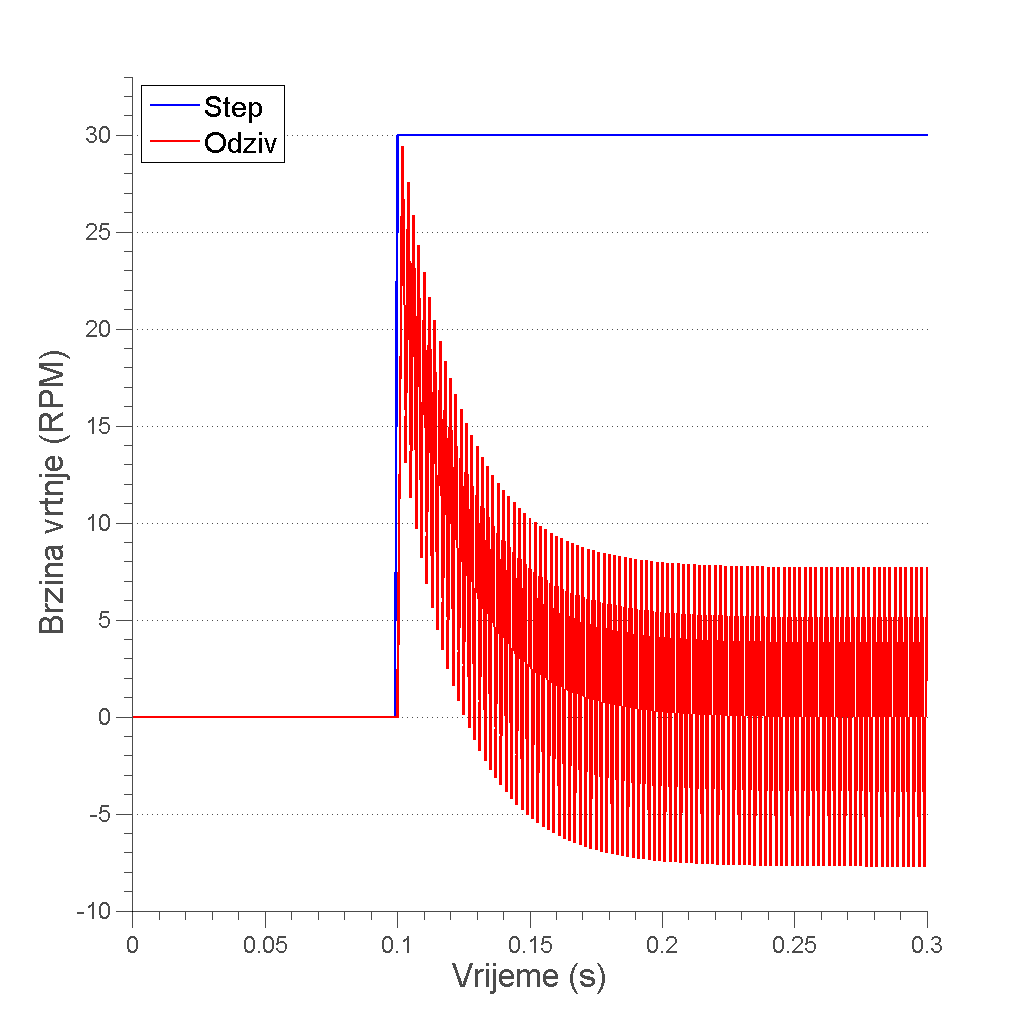
\includegraphics[width=0.8\textwidth] {odziv_2.png}
    \caption{Odziv sustava $C(s)\cdot K_p\cdot G_p(s)$ na skokovitu pobudu}
    \end{center}
\end{figure}


Primjećujemo da sustav ima poprilično odstupanje od referentnog signala te da oscilira oko vrijednosti tog odstupanja. Očito naš sustav ne može dobro pratiti signal step funkcije kada proces nije reguliran dodatnim integracijskim članom.


\newpage

Uspoređujemo li referentni i regulirani signal brzine vrtnje kod skokovite pobude pri deset puta većem pojačanju $K_p$, dobivamo sljedeći odziv, kao što je prikazan na slici 2.10.


\begin{figure}[h]
	\begin{center}
	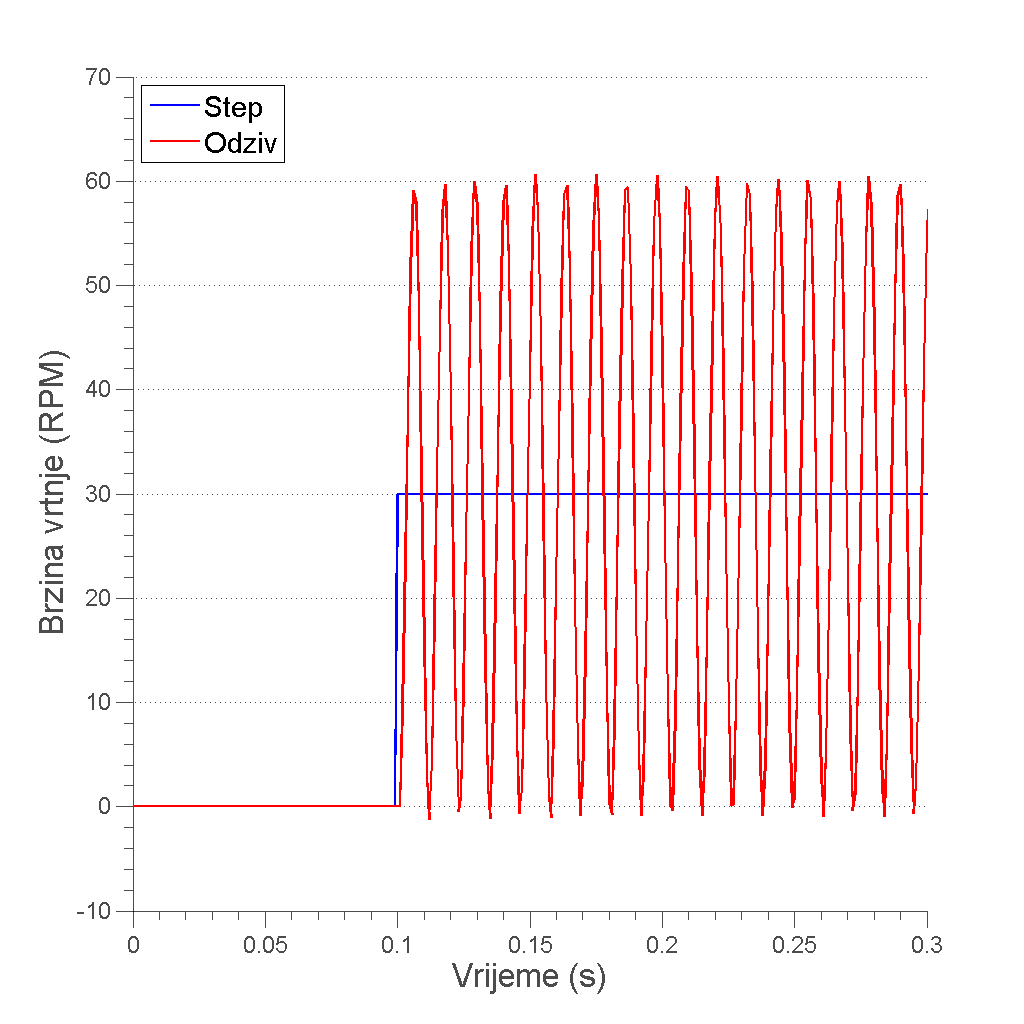
\includegraphics[width=0.8\textwidth] {odziv_3.png}
    \caption{Odziv sustava $C(s)\cdot K_p\cdot G_p(s)/s$ na skokovitu pobudu pri $K_p$ = 415.5}
    \end{center}
\end{figure}

Ukoliko povećamo statičko pojačanje $K_p$, sustav će brže pratiti referentnu veličinu, no iz tog razloga može postati nestabilan, što se i vidi iz slike 2.10. Zbog nestabilnosti sustav oscilira i do pune vrijednosti amplitude.


\newpage

U slučaju kada sustav umjesto negativne povratne veze ima pozitivnu povratnu vezu, odziv sustava vlada se prema formuli

\begin{equation}
Y(s)=\frac{G_r(s)\cdot G_p(s)}{1 - G_r(s)\cdot G_p(s)}R_p(s)
\end{equation}

gdje su $ G_r(s)=C(s)\cdot K_p \cdot \frac{1}{s}$ i $ G_p(s)$ naš regulator, odnosno proces sustava.

Kako od pojave step funkcije svako pojačanje sustava doprinosi dodatnom pojačanju ulaza u sustav, rast izlazne veličine sustava je eksponecijalan, što se lako uočava na slici 2.11.

\begin{figure}[h]
	\begin{center}
	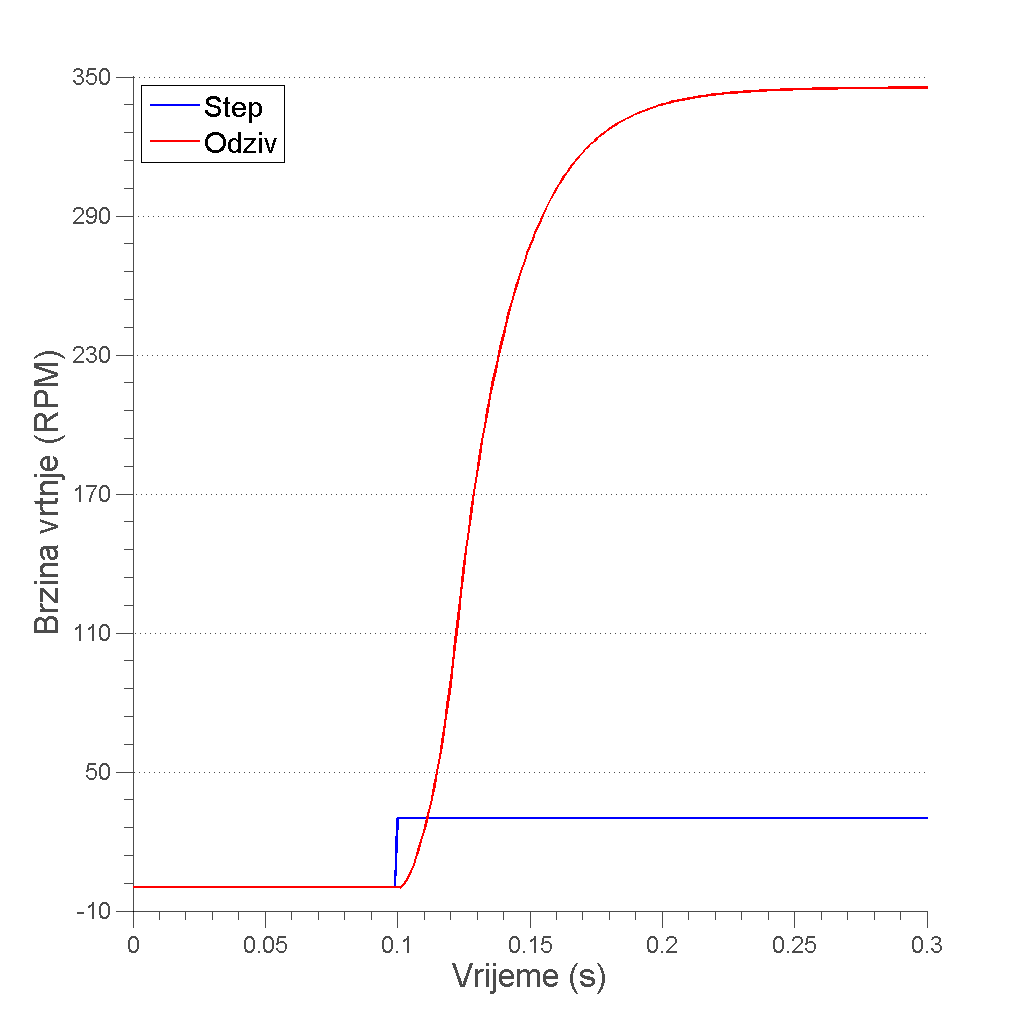
\includegraphics[width=0.8\textwidth] {odziv_4.png}
    \caption{Odziv sustava $C(s)\cdot K_p\cdot G_p(s)/s$ na skokovitu pobudu sa pozitivnom povratnom vezom}
    \end{center}
\end{figure}

Jedini razlog zašto odziv brzine vrtnje usporava svoj rast i naposljetku se stabilizira oko određene veličine je jer naš matematički model rotacijskog eletktromehaničkog modula SRV02, odnosno u ovom sustavu proces, ima definiran limitator ulazne veličine na iznose između $[-6, 6]$ V, te je time naš model nelinearan.


\newpage

Ukoliko promatramo odziv sustava za slučaj kada je prekinuta povratna veza u potpunosti, dobivamo odziv kakav je prikazan na slici 2.12.

\begin{figure}[h]
	\begin{center}
	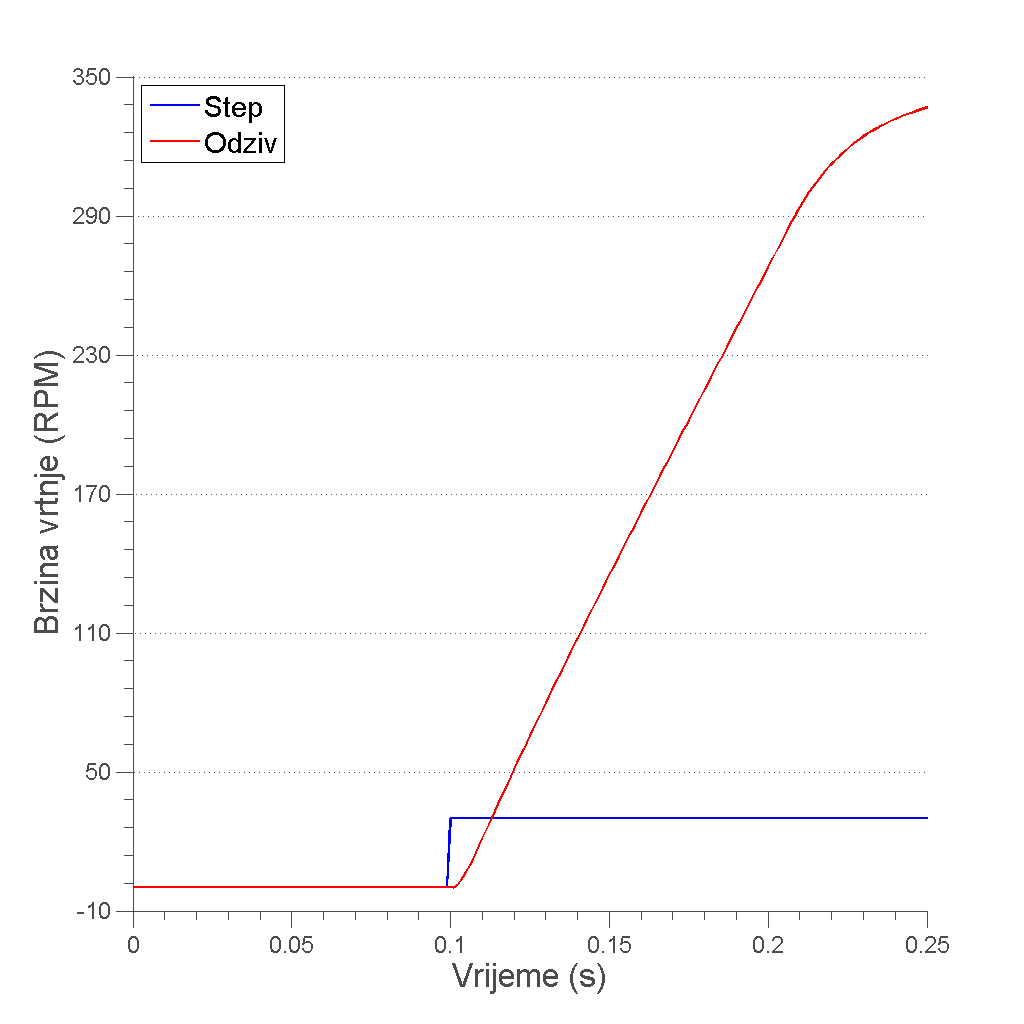
\includegraphics[width=0.8\textwidth] {odziv_5.png}
    \caption{Odziv sustava $C(s)\cdot K_p\cdot G_p(s)/s$ na skokovitu pobudu bez povratne veze}
    \end{center}
\end{figure}

Primjećujemo da odziv sustava konstantno raste, jer bez povratne veze sustava nije moguće regulirati sa zadanim regulatorom $G_r(s)$. Na kraju krivulje možemo primjetiti da se odziv ponovo stabilizira i to iz istog razloga kao i kod prijašnjeg odziva.

\newpage


\subsubsection{Opažanja i zaključci}
Tokom simulacije ovoga sustava koristili smo prije definirane elemente regulatora $ G_r(s)=C(s)\cdot K_p \cdot \frac{1}{s}$, koji unutar sebe sadrži statičko pojačanje, integracijski i kompenzacijsko derivacijski član, te sam proces sustava $ G_p(s)$ kojeg smo stvorili pomoću matematičkog modela.

S obzirom da smo unutar matematičkog modela procesa sustava uvrstili limitator ulazne veličine, koji je nužan da simuliramo stvarne limitacije ulaznog napona na rotacijski elektromehanički modul SRV02, time smo zapravo naš linearni matematički model učinili nelinearnim.

Zbog te nelinearnosti našeg matematičkog modela procesa sustava mogli bismo očekivati probleme pri izvođenju simulacije. Konkretno, moguće je pojavljivanje trajnog regulacijskog odstupanja, što smo i primjetili u zadnja dva mjerenja, te su moguće pojave dodatnih frekvencija unutar kruga u slučaju periodičke funkcije i slično.


Pored tih nedostataka, uvođenjem nelinearnosti vjernije smo modelirali limitacije našeg rotacijskog elektromehaničkog modula, ali trebamo imati na umu te adaptacije matematičkog modela pri daljnim simulacijama.


Možemo zaključiti da je, u svrhu ovih simulacija, naš model procesa i regulatora bio adekvatan.

\end{document}


%Na vlastitu odgovornost...
